\section{Data yang dipakai}\label{sec:data}
\subsection{Semua data perdagangan adalah milik Indonesia}
Sumber perdagangan adalah 22 workbook Trade Map dari pengguna: ekspor dan impor Indonesia dengan sepuluh mitra, ditambah ekspor dan impor Indonesia dengan seluruh negara. Pada file ekspor, Indonesia adalah eksportir. Pada file impor, Indonesia adalah importir.

Pemeriksaan metadata menunjukkan kode pelapor 360, yaitu Indonesia, pada semua workbook. Kode 000 atau \texttt{World} pada file total berarti semua negara mitra. Jadi, data ini tidak menjumlahkan perdagangan antarsemua negara di dunia.

Sebanyak 5.456 angka TOTAL bulanan sudah dicocokkan dengan dataset hasil pengolahan dan semuanya sesuai. Pemeriksaan ini memastikan bahwa data diambil dan diolah dari file yang benar. Pemeriksaan tersebut belum sama dengan membandingkan setiap angka terhadap sumber statistik nasional yang independen.

Dalam dataset, kolom \texttt{ISO3} berisi kode mitra. \texttt{CHN} berarti Tiongkok sebagai mitra Indonesia; \texttt{WLD} berarti seluruh mitra Indonesia. Pada data kelompok barang, nama kelompok menjadi kunci tambahan.

\subsection{Dari data bulanan menjadi kuartalan}
Workbook berisi nilai bulanan Januari 2006--Agustus 2026 dalam USD ribu. Ekspor dan impor dijumlahkan untuk membentuk data kuartalan. Satu kuartal hanya dipakai sebagai kuartal lengkap bila ketiga bulannya tersedia. Juli--Agustus 2026 belum cukup untuk membentuk kuartal ketiga lengkap.

Angka nol yang memang tertulis pada file tetap menjadi nol. Sel kosong tidak otomatis dianggap nol. Pada nilai perdagangan yang diimpor untuk run ini, pemeriksaan tidak menemukan sel numerik yang kosong.

Untuk total Indonesia dan total per mitra, perhitungan memakai baris TOTAL dari workbook. Untuk kelompok barang, nilainya dijumlahkan dari kode HS-6 yang masuk kelompok tersebut. Jumlah seluruh rincian produk juga dibandingkan dengan TOTAL.

Selisih kecil bisa muncul karena angka per produk dibulatkan. Selisih relatif maksimum yang tercatat sekitar 0,0483\%, dan semuanya masih berada dalam batas pembulatan yang dipakai. Jadi, selisih tersebut tidak langsung dianggap sebagai produk yang hilang.

Nilai dalam grafik tahunan dikonversi ke USD miliar. Pada 2025, ekspor Indonesia mencapai USD \WorldExports{} miliar, impor USD \WorldImports{} miliar, dan surplus USD \WorldNet{} miliar. Tahun 2025 dipakai untuk melihat struktur perdagangan karena datanya lengkap.

\begin{figure}[!htbp]\centering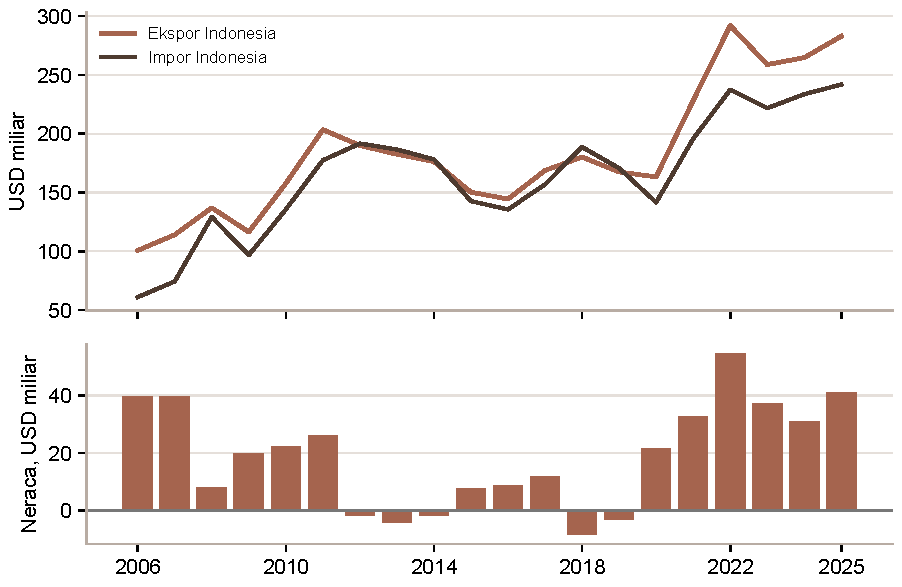
\includegraphics[width=\linewidth]{assets/indonesia_annual.pdf}
\caption{Ekspor, impor, dan trade balance Indonesia dengan seluruh negara. Grafik tahunan hanya memakai tahun dengan empat kuartal lengkap. Sumber: data Trade Map pengguna.}\label{fig:annual}
\end{figure}

\subsection{Mengapa ada tujuh kelompok barang?}
Ada dua cara pengelompokan yang dipakai. Cara pertama membedakan komoditas dari manufaktur nonkomoditas, mengikuti kelompok A11 UNCTAD melalui mapping HS--SITC \cite{unctad,unsdcorr}. Komoditas total kemudian dirinci menjadi pertanian/pangan dan energi/tambang.

Cara kedua melihat penggunaan barang: konsumsi, modal, atau bahan baku/penolong. Ini mengikuti BEC Rev.5 \cite{bec}. Kedua cara tersebut menjawab pertanyaan yang berbeda. Sebuah komoditas bisa menjadi barang konsumsi atau bahan baku. Barang manufaktur juga bisa menjadi barang modal atau input produksi.

\begin{table}[!htbp]\centering\small
\caption{Arti tujuh kelompok barang}
\begin{tabular}{p{.07\linewidth}p{.29\linewidth}p{.53\linewidth}}
\toprule Kode & Kelompok & Penjelasan\\\midrule
G1 & Manufaktur nonkomoditas & Barang nonkomoditas menurut mapping UNCTAD yang dipakai.\\
G2 & Barang konsumsi & Barang untuk konsumsi akhir menurut BEC Rev.5.\\
G3 & Pertanian dan pangan & Komoditas pangan dan bahan mentah pertanian.\\
G4 & Bahan baku/penolong & Barang untuk penggunaan antara dalam produksi.\\
G5 & Barang modal & Barang untuk pembentukan modal tetap.\\
G6 & Komoditas total & Semua komoditas A11 yang berhasil dipetakan.\\
G7 & Energi dan tambang & Bahan bakar, bijih/mineral, dan komoditas logam terkait.\\
\bottomrule\end{tabular}\label{tab:groups}
\end{table}

\textbf{Ketujuh kelompok tidak boleh dijumlahkan menjadi total perdagangan.} Sebagian nilainya masuk ke lebih dari satu kelompok karena cara pengelompokannya berbeda. Hasil regresi kelompok yang tumpang tindih juga tidak bisa dihitung sebagai bukti yang sepenuhnya independen.

Ada masalah lain yang belum selesai: workbook tidak menyebut versi HS untuk setiap angka. Kode yang sama bisa mempunyai mapping berbeda pada revisi yang berbeda. Karena itu, suatu kode hanya dimasukkan ke kelompok tertentu bila mapping resminya konsisten. Kode yang masih ambigu dibiarkan sebagai campuran atau belum terpetakan.

Nilai kode yang ambigu tetap masuk dalam TOTAL, tetapi tidak dipaksakan masuk ke kelompok yang belum jelas. Cara ini lebih hati-hati, namun belum membuat produk sepenuhnya sebanding dari tahun ke tahun. Hasil kelompok juga belum tentu berlaku untuk setiap produk atau perusahaan di dalamnya.

\subsection{Data GDP, kurs, dan harga}
Model memasukkan aktivitas ekonomi Indonesia dan negara mitra. Ukurannya adalah level \emph{real GDP}, atau PDB riil, yang diubah menjadi indeks lalu di-log. Ini berbeda dari memasukkan pertumbuhan GDP tahunan.

Untuk total perdagangan Indonesia, aktivitas luar negeri diwakili oleh gabungan real GDP sepuluh mitra dengan bobot ekspor tetap 2006--2008. Ini adalah proksi permintaan luar negeri. Angkanya tidak sama dengan GDP seluruh dunia.

Kurs total Indonesia menggunakan REER BIS. Kurs bilateral dibentuk dari kurs nominal dan indeks harga. Arahnya dibuat sama: angka kurs yang naik berarti apresiasi. Jadi, perubahan yang diuji adalah perubahan kurs riil, bukan otomatis perubahan rupiah terhadap dolar dengan besaran yang sama.

Indeks harga komoditas BCOM ditambahkan pada beberapa model pembanding. Tujuannya melihat apakah hasil berubah ketika satu ukuran harga global ikut dimasukkan. BCOM tidak langsung mengukur harga semua produk HS-6.

\subsection{Mengapa periode data tiap negara berbeda?}
Model hanya memakai rentang kuartal terpanjang yang lengkap. Jika ada kuartal kosong, kuartal sebelum dan sesudahnya tidak disambung seolah tidak ada jeda. Ini menjaga arti lag, yaitu jarak waktu dalam model.

Data CPI India yang dipakai baseline mulai 2013. CPI Australia bulanan memuat interpolasi dari penyedia. CPI AS Oktober 2025 dan kurs Vietnam Agustus 2025 kosong pada seri utama. Ada pula catatan tentang versi historis GDP dan perbedaan definisi kurs antarpenyedia. Karena itu, rentang estimasi tiap mitra tidak selalu sama.

Untuk total Indonesia, baseline dimulai dari data 2010Q1 agar bisa dibandingkan dengan run sebelumnya. Setelah empat lag disiapkan, regresinya memakai 2011Q1--2026Q1. Model dengan data mulai 2006 tetap dijalankan sebagai robustness check.

\begin{table}[!htbp]\centering\caption{Gambaran sampel total Indonesia, 2011Q1--2026Q1}
{\small\setlength{\tabcolsep}{3pt}\renewcommand{\arraystretch}{1.15}
\begin{tabular}{p{0.32\linewidth}p{0.045\linewidth}p{0.12\linewidth}p{0.12\linewidth}p{0.12\linewidth}p{0.12\linewidth}}
\toprule
\textbf{Variabel} & \textbf{N} & \textbf{Rerata} & \textbf{SD} & \textbf{Min.} & \textbf{Maks.}\\
\midrule
Ekspor, USD miliar & 61 & 51,15 & 12,46 & 33,60 & 78,20\\
Impor, USD miliar & 61 & 46,92 & 9,06 & 31,73 & 65,54\\
Neraca, USD miliar & 61 & 4,24 & 5,08 & -4,80 & 15,61\\
PDB riil Indonesia, indeks & 61 & 114,85 & 21,27 & 79,40 & 156,49\\
Aktivitas luar negeri, indeks & 61 & 109,43 & 13,98 & 86,16 & 135,66\\
REER, indeks & 61 & 100,99 & 4,32 & 92,89 & 111,01\\
\bottomrule
\end{tabular}
}\label{tab:desc}
\end{table}

Pada tabel ini, ekspor dan impor adalah nilai per kuartal. N berarti jumlah kuartal. SD adalah standard deviation, yaitu ukuran seberapa besar data bervariasi di sekitar rata-ratanya. Meski rata-rata trade balance positif, tetap ada kuartal defisit.

Perdagangan belum disesuaikan secara musiman. Sebagian GDP memakai seri penyedia yang sudah disesuaikan. Perbedaan ini masih perlu diperiksa dalam pengembangan model berikutnya.
